% Created by tikzDevice version 0.10.1 on 2020-02-15 15:52:16
% !TEX encoding = UTF-8 Unicode
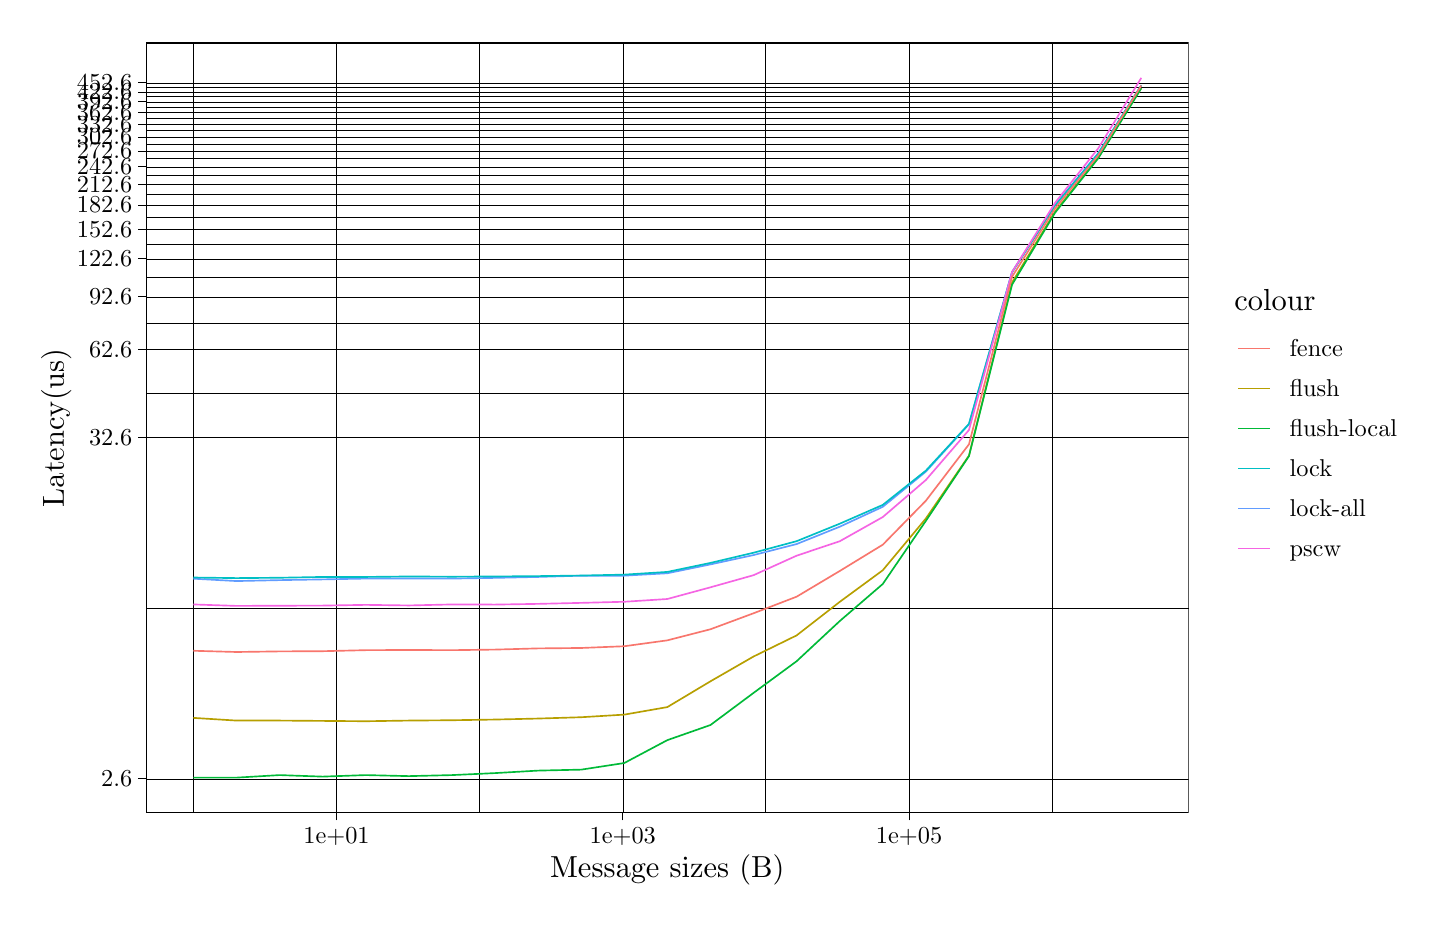
\begin{tikzpicture}[x=1pt,y=1pt]
\definecolor{fillColor}{RGB}{255,255,255}
\path[use as bounding box,fill=fillColor,fill opacity=0.00] (0,0) rectangle (505.89,314.37);
\begin{scope}
\path[clip] (  0.00,  0.00) rectangle (505.89,314.37);
\definecolor{drawColor}{RGB}{255,255,255}
\definecolor{fillColor}{RGB}{255,255,255}

\path[draw=drawColor,line width= 0.6pt,line join=round,line cap=round,fill=fillColor] (  0.00,  0.00) rectangle (505.89,314.37);
\end{scope}
\begin{scope}
\path[clip] ( 42.76, 30.72) rectangle (419.53,308.87);
\definecolor{fillColor}{RGB}{255,255,255}

\path[fill=fillColor] ( 42.76, 30.72) rectangle (419.53,308.87);
\definecolor{drawColor}{RGB}{0,0,0}

\path[draw=drawColor,line width= 0.0pt,line join=round] ( 42.76,104.63) --
	(419.53,104.63);

\path[draw=drawColor,line width= 0.0pt,line join=round] ( 42.76,182.16) --
	(419.53,182.16);

\path[draw=drawColor,line width= 0.0pt,line join=round] ( 42.76,207.61) --
	(419.53,207.61);

\path[draw=drawColor,line width= 0.0pt,line join=round] ( 42.76,223.99) --
	(419.53,223.99);

\path[draw=drawColor,line width= 0.0pt,line join=round] ( 42.76,236.16) --
	(419.53,236.16);

\path[draw=drawColor,line width= 0.0pt,line join=round] ( 42.76,245.87) --
	(419.53,245.87);

\path[draw=drawColor,line width= 0.0pt,line join=round] ( 42.76,253.96) --
	(419.53,253.96);

\path[draw=drawColor,line width= 0.0pt,line join=round] ( 42.76,260.88) --
	(419.53,260.88);

\path[draw=drawColor,line width= 0.0pt,line join=round] ( 42.76,266.94) --
	(419.53,266.94);

\path[draw=drawColor,line width= 0.0pt,line join=round] ( 42.76,272.32) --
	(419.53,272.32);

\path[draw=drawColor,line width= 0.0pt,line join=round] ( 42.76,277.17) --
	(419.53,277.17);

\path[draw=drawColor,line width= 0.0pt,line join=round] ( 42.76,281.58) --
	(419.53,281.58);

\path[draw=drawColor,line width= 0.0pt,line join=round] ( 42.76,285.62) --
	(419.53,285.62);

\path[draw=drawColor,line width= 0.0pt,line join=round] ( 42.76,289.36) --
	(419.53,289.36);

\path[draw=drawColor,line width= 0.0pt,line join=round] ( 42.76,292.82) --
	(419.53,292.82);

\path[draw=drawColor,line width= 0.0pt,line join=round] ( 59.89, 30.72) --
	( 59.89,308.87);

\path[draw=drawColor,line width= 0.0pt,line join=round] (163.32, 30.72) --
	(163.32,308.87);

\path[draw=drawColor,line width= 0.0pt,line join=round] (266.76, 30.72) --
	(266.76,308.87);

\path[draw=drawColor,line width= 0.0pt,line join=round] (370.20, 30.72) --
	(370.20,308.87);

\path[draw=drawColor,line width= 0.1pt,line join=round] ( 42.76, 42.99) --
	(419.53, 42.99);

\path[draw=drawColor,line width= 0.1pt,line join=round] ( 42.76,166.26) --
	(419.53,166.26);

\path[draw=drawColor,line width= 0.1pt,line join=round] ( 42.76,198.06) --
	(419.53,198.06);

\path[draw=drawColor,line width= 0.1pt,line join=round] ( 42.76,217.15) --
	(419.53,217.15);

\path[draw=drawColor,line width= 0.1pt,line join=round] ( 42.76,230.83) --
	(419.53,230.83);

\path[draw=drawColor,line width= 0.1pt,line join=round] ( 42.76,241.50) --
	(419.53,241.50);

\path[draw=drawColor,line width= 0.1pt,line join=round] ( 42.76,250.25) --
	(419.53,250.25);

\path[draw=drawColor,line width= 0.1pt,line join=round] ( 42.76,257.66) --
	(419.53,257.66);

\path[draw=drawColor,line width= 0.1pt,line join=round] ( 42.76,264.10) --
	(419.53,264.10);

\path[draw=drawColor,line width= 0.1pt,line join=round] ( 42.76,269.78) --
	(419.53,269.78);

\path[draw=drawColor,line width= 0.1pt,line join=round] ( 42.76,274.87) --
	(419.53,274.87);

\path[draw=drawColor,line width= 0.1pt,line join=round] ( 42.76,279.48) --
	(419.53,279.48);

\path[draw=drawColor,line width= 0.1pt,line join=round] ( 42.76,283.69) --
	(419.53,283.69);

\path[draw=drawColor,line width= 0.1pt,line join=round] ( 42.76,287.56) --
	(419.53,287.56);

\path[draw=drawColor,line width= 0.1pt,line join=round] ( 42.76,291.15) --
	(419.53,291.15);

\path[draw=drawColor,line width= 0.1pt,line join=round] ( 42.76,294.49) --
	(419.53,294.49);

\path[draw=drawColor,line width= 0.1pt,line join=round] (111.60, 30.72) --
	(111.60,308.87);

\path[draw=drawColor,line width= 0.1pt,line join=round] (215.04, 30.72) --
	(215.04,308.87);

\path[draw=drawColor,line width= 0.1pt,line join=round] (318.48, 30.72) --
	(318.48,308.87);
\definecolor{drawColor}{RGB}{97,156,255}

\path[draw=drawColor,line width= 0.6pt,line join=round] ( 59.89,115.26) --
	( 75.45,114.40) --
	( 91.02,114.74) --
	(106.59,115.00) --
	(122.16,115.30) --
	(137.73,115.30) --
	(153.30,115.30) --
	(168.87,115.55) --
	(184.44,115.89) --
	(200.01,116.35) --
	(215.58,116.35) --
	(231.14,117.22) --
	(246.71,120.42) --
	(262.28,123.79) --
	(277.85,127.77) --
	(293.42,134.03) --
	(308.99,141.24) --
	(324.56,153.94) --
	(340.13,171.08) --
	(355.70,226.09) --
	(371.27,250.28) --
	(386.83,268.98) --
	(402.40,293.57);
\definecolor{drawColor}{RGB}{0,191,196}

\path[draw=drawColor,line width= 0.6pt,line join=round] ( 59.89,115.68) --
	( 75.45,115.47) --
	( 91.02,115.60) --
	(106.59,115.89) --
	(122.16,115.89) --
	(137.73,116.06) --
	(153.30,115.98) --
	(168.87,116.06) --
	(184.44,116.19) --
	(200.01,116.39) --
	(215.58,116.73) --
	(231.14,117.71) --
	(246.71,120.96) --
	(262.28,124.64) --
	(277.85,128.81) --
	(293.42,135.12) --
	(308.99,141.93) --
	(324.56,154.31) --
	(340.13,171.20) --
	(355.70,225.95) --
	(371.27,250.18) --
	(386.83,268.88) --
	(402.40,293.50);
\definecolor{drawColor}{RGB}{183,159,0}

\path[draw=drawColor,line width= 0.6pt,line join=round] ( 59.89, 64.96) --
	( 75.45, 63.99) --
	( 91.02, 63.99) --
	(106.59, 63.87) --
	(122.16, 63.75) --
	(137.73, 63.99) --
	(153.30, 64.11) --
	(168.87, 64.36) --
	(184.44, 64.72) --
	(200.01, 65.20) --
	(215.58, 66.14) --
	(231.14, 68.86) --
	(246.71, 78.17) --
	(262.28, 87.13) --
	(277.85, 94.76) --
	(293.42,106.87) --
	(308.99,118.31) --
	(324.56,137.01) --
	(340.13,159.74) --
	(355.70,222.30) --
	(371.27,247.94) --
	(386.83,267.41) --
	(402.40,292.60);
\definecolor{drawColor}{RGB}{0,186,56}

\path[draw=drawColor,line width= 0.6pt,line join=round] ( 59.89, 43.37) --
	( 75.45, 43.37) --
	( 91.02, 44.29) --
	(106.59, 43.74) --
	(122.16, 44.29) --
	(137.73, 43.92) --
	(153.30, 44.29) --
	(168.87, 45.01) --
	(184.44, 45.91) --
	(200.01, 46.26) --
	(215.58, 48.65) --
	(231.14, 56.92) --
	(246.71, 62.38) --
	(262.28, 73.98) --
	(277.85, 85.43) --
	(293.42, 99.93) --
	(308.99,113.35) --
	(324.56,136.16) --
	(340.13,159.55) --
	(355.70,221.49) --
	(371.27,247.53) --
	(386.83,267.16) --
	(402.40,292.48);
\definecolor{drawColor}{RGB}{245,100,227}

\path[draw=drawColor,line width= 0.6pt,line join=round] ( 59.89,105.95) --
	( 75.45,105.43) --
	( 91.02,105.49) --
	(106.59,105.54) --
	(122.16,105.80) --
	(137.73,105.59) --
	(153.30,105.95) --
	(168.87,105.90) --
	(184.44,106.16) --
	(200.01,106.52) --
	(215.58,106.92) --
	(231.14,107.92) --
	(246.71,112.14) --
	(262.28,116.52) --
	(277.85,123.57) --
	(293.42,128.78) --
	(308.99,137.53) --
	(324.56,150.92) --
	(340.13,168.98) --
	(355.70,226.05) --
	(371.27,251.12) --
	(386.83,270.73) --
	(402.40,296.23);
\definecolor{drawColor}{RGB}{248,118,109}

\path[draw=drawColor,line width= 0.6pt,line join=round] ( 59.89, 89.21) --
	( 75.45, 88.77) --
	( 91.02, 88.99) --
	(106.59, 89.06) --
	(122.16, 89.43) --
	(137.73, 89.50) --
	(153.30, 89.43) --
	(168.87, 89.64) --
	(184.44, 90.07) --
	(200.01, 90.22) --
	(215.58, 90.85) --
	(231.14, 92.98) --
	(246.71, 96.98) --
	(262.28,102.76) --
	(277.85,108.75) --
	(293.42,118.03) --
	(308.99,127.54) --
	(324.56,143.43) --
	(340.13,163.81) --
	(355.70,224.35) --
	(371.27,249.11) --
	(386.83,268.21) --
	(402.40,293.47);
\definecolor{drawColor}{RGB}{0,0,0}

\path[draw=drawColor,line width= 0.6pt,line join=round,line cap=round] ( 42.76, 30.72) rectangle (419.53,308.87);
\end{scope}
\begin{scope}
\path[clip] (  0.00,  0.00) rectangle (505.89,314.37);
\definecolor{drawColor}{RGB}{0,0,0}

\node[text=drawColor,anchor=base west,inner sep=0pt, outer sep=0pt, scale=  0.88] at ( 26.57, 40.17) {2.6};

\node[text=drawColor,anchor=base west,inner sep=0pt, outer sep=0pt, scale=  0.88] at ( 22.17,163.44) {32.6};

\node[text=drawColor,anchor=base west,inner sep=0pt, outer sep=0pt, scale=  0.88] at ( 22.17,195.24) {62.6};

\node[text=drawColor,anchor=base west,inner sep=0pt, outer sep=0pt, scale=  0.88] at ( 22.17,214.33) {92.6};

\node[text=drawColor,anchor=base west,inner sep=0pt, outer sep=0pt, scale=  0.88] at ( 17.77,228.01) {122.6};

\node[text=drawColor,anchor=base west,inner sep=0pt, outer sep=0pt, scale=  0.88] at ( 17.77,238.68) {152.6};

\node[text=drawColor,anchor=base west,inner sep=0pt, outer sep=0pt, scale=  0.88] at ( 17.77,247.43) {182.6};

\node[text=drawColor,anchor=base west,inner sep=0pt, outer sep=0pt, scale=  0.88] at ( 17.77,254.84) {212.6};

\node[text=drawColor,anchor=base west,inner sep=0pt, outer sep=0pt, scale=  0.88] at ( 17.77,261.27) {242.6};

\node[text=drawColor,anchor=base west,inner sep=0pt, outer sep=0pt, scale=  0.88] at ( 17.77,266.96) {272.6};

\node[text=drawColor,anchor=base west,inner sep=0pt, outer sep=0pt, scale=  0.88] at ( 17.77,272.05) {302.6};

\node[text=drawColor,anchor=base west,inner sep=0pt, outer sep=0pt, scale=  0.88] at ( 17.77,276.65) {332.6};

\node[text=drawColor,anchor=base west,inner sep=0pt, outer sep=0pt, scale=  0.88] at ( 17.77,280.86) {362.6};

\node[text=drawColor,anchor=base west,inner sep=0pt, outer sep=0pt, scale=  0.88] at ( 17.77,284.74) {392.6};

\node[text=drawColor,anchor=base west,inner sep=0pt, outer sep=0pt, scale=  0.88] at ( 17.77,288.33) {422.6};

\node[text=drawColor,anchor=base west,inner sep=0pt, outer sep=0pt, scale=  0.88] at ( 17.77,291.67) {452.6};
\end{scope}
\begin{scope}
\path[clip] (  0.00,  0.00) rectangle (505.89,314.37);
\definecolor{drawColor}{RGB}{0,0,0}

\path[draw=drawColor,line width= 0.3pt,line join=round] ( 40.01, 42.99) --
	( 42.76, 42.99);

\path[draw=drawColor,line width= 0.3pt,line join=round] ( 40.01,166.26) --
	( 42.76,166.26);

\path[draw=drawColor,line width= 0.3pt,line join=round] ( 40.01,198.06) --
	( 42.76,198.06);

\path[draw=drawColor,line width= 0.3pt,line join=round] ( 40.01,217.15) --
	( 42.76,217.15);

\path[draw=drawColor,line width= 0.3pt,line join=round] ( 40.01,230.83) --
	( 42.76,230.83);

\path[draw=drawColor,line width= 0.3pt,line join=round] ( 40.01,241.50) --
	( 42.76,241.50);

\path[draw=drawColor,line width= 0.3pt,line join=round] ( 40.01,250.25) --
	( 42.76,250.25);

\path[draw=drawColor,line width= 0.3pt,line join=round] ( 40.01,257.66) --
	( 42.76,257.66);

\path[draw=drawColor,line width= 0.3pt,line join=round] ( 40.01,264.10) --
	( 42.76,264.10);

\path[draw=drawColor,line width= 0.3pt,line join=round] ( 40.01,269.78) --
	( 42.76,269.78);

\path[draw=drawColor,line width= 0.3pt,line join=round] ( 40.01,274.87) --
	( 42.76,274.87);

\path[draw=drawColor,line width= 0.3pt,line join=round] ( 40.01,279.48) --
	( 42.76,279.48);

\path[draw=drawColor,line width= 0.3pt,line join=round] ( 40.01,283.69) --
	( 42.76,283.69);

\path[draw=drawColor,line width= 0.3pt,line join=round] ( 40.01,287.56) --
	( 42.76,287.56);

\path[draw=drawColor,line width= 0.3pt,line join=round] ( 40.01,291.15) --
	( 42.76,291.15);

\path[draw=drawColor,line width= 0.3pt,line join=round] ( 40.01,294.49) --
	( 42.76,294.49);
\end{scope}
\begin{scope}
\path[clip] (  0.00,  0.00) rectangle (505.89,314.37);
\definecolor{drawColor}{RGB}{0,0,0}

\path[draw=drawColor,line width= 0.3pt,line join=round] (111.60, 27.97) --
	(111.60, 30.72);

\path[draw=drawColor,line width= 0.3pt,line join=round] (215.04, 27.97) --
	(215.04, 30.72);

\path[draw=drawColor,line width= 0.3pt,line join=round] (318.48, 27.97) --
	(318.48, 30.72);
\end{scope}
\begin{scope}
\path[clip] (  0.00,  0.00) rectangle (505.89,314.37);
\definecolor{drawColor}{RGB}{0,0,0}

\node[text=drawColor,anchor=base,inner sep=0pt, outer sep=0pt, scale=  0.88] at (111.60, 19.71) {1e+01};

\node[text=drawColor,anchor=base,inner sep=0pt, outer sep=0pt, scale=  0.88] at (215.04, 19.71) {1e+03};

\node[text=drawColor,anchor=base,inner sep=0pt, outer sep=0pt, scale=  0.88] at (318.48, 19.71) {1e+05};
\end{scope}
\begin{scope}
\path[clip] (  0.00,  0.00) rectangle (505.89,314.37);
\definecolor{drawColor}{RGB}{0,0,0}

\node[text=drawColor,anchor=base,inner sep=0pt, outer sep=0pt, scale=  1.10] at (231.14,  7.44) {Message sizes (B)};
\end{scope}
\begin{scope}
\path[clip] (  0.00,  0.00) rectangle (505.89,314.37);
\definecolor{drawColor}{RGB}{0,0,0}

\node[text=drawColor,rotate= 90.00,anchor=base,inner sep=0pt, outer sep=0pt, scale=  1.10] at ( 13.08,169.80) {Latency(us)};
\end{scope}
\begin{scope}
\path[clip] (  0.00,  0.00) rectangle (505.89,314.37);
\definecolor{fillColor}{RGB}{255,255,255}

\path[fill=fillColor] (430.53,113.43) rectangle (500.39,226.17);
\end{scope}
\begin{scope}
\path[clip] (  0.00,  0.00) rectangle (505.89,314.37);
\definecolor{drawColor}{RGB}{0,0,0}

\node[text=drawColor,anchor=base west,inner sep=0pt, outer sep=0pt, scale=  1.10] at (436.03,212.12) {colour};
\end{scope}
\begin{scope}
\path[clip] (  0.00,  0.00) rectangle (505.89,314.37);
\definecolor{fillColor}{RGB}{255,255,255}

\path[fill=fillColor] (436.03,191.20) rectangle (450.48,205.65);
\end{scope}
\begin{scope}
\path[clip] (  0.00,  0.00) rectangle (505.89,314.37);
\definecolor{drawColor}{RGB}{248,118,109}

\path[draw=drawColor,line width= 0.6pt,line join=round] (437.48,198.42) -- (449.04,198.42);
\end{scope}
\begin{scope}
\path[clip] (  0.00,  0.00) rectangle (505.89,314.37);
\definecolor{drawColor}{RGB}{248,118,109}

\path[draw=drawColor,line width= 0.6pt,line join=round] (437.48,198.42) -- (449.04,198.42);
\end{scope}
\begin{scope}
\path[clip] (  0.00,  0.00) rectangle (505.89,314.37);
\definecolor{drawColor}{RGB}{248,118,109}

\path[draw=drawColor,line width= 0.6pt,line join=round] (437.48,198.42) -- (449.04,198.42);
\end{scope}
\begin{scope}
\path[clip] (  0.00,  0.00) rectangle (505.89,314.37);
\definecolor{drawColor}{RGB}{248,118,109}

\path[draw=drawColor,line width= 0.6pt,line join=round] (437.48,198.42) -- (449.04,198.42);
\end{scope}
\begin{scope}
\path[clip] (  0.00,  0.00) rectangle (505.89,314.37);
\definecolor{drawColor}{RGB}{248,118,109}

\path[draw=drawColor,line width= 0.6pt,line join=round] (437.48,198.42) -- (449.04,198.42);
\end{scope}
\begin{scope}
\path[clip] (  0.00,  0.00) rectangle (505.89,314.37);
\definecolor{drawColor}{RGB}{248,118,109}

\path[draw=drawColor,line width= 0.6pt,line join=round] (437.48,198.42) -- (449.04,198.42);
\end{scope}
\begin{scope}
\path[clip] (  0.00,  0.00) rectangle (505.89,314.37);
\definecolor{fillColor}{RGB}{255,255,255}

\path[fill=fillColor] (436.03,176.74) rectangle (450.48,191.20);
\end{scope}
\begin{scope}
\path[clip] (  0.00,  0.00) rectangle (505.89,314.37);
\definecolor{drawColor}{RGB}{183,159,0}

\path[draw=drawColor,line width= 0.6pt,line join=round] (437.48,183.97) -- (449.04,183.97);
\end{scope}
\begin{scope}
\path[clip] (  0.00,  0.00) rectangle (505.89,314.37);
\definecolor{drawColor}{RGB}{183,159,0}

\path[draw=drawColor,line width= 0.6pt,line join=round] (437.48,183.97) -- (449.04,183.97);
\end{scope}
\begin{scope}
\path[clip] (  0.00,  0.00) rectangle (505.89,314.37);
\definecolor{drawColor}{RGB}{183,159,0}

\path[draw=drawColor,line width= 0.6pt,line join=round] (437.48,183.97) -- (449.04,183.97);
\end{scope}
\begin{scope}
\path[clip] (  0.00,  0.00) rectangle (505.89,314.37);
\definecolor{drawColor}{RGB}{183,159,0}

\path[draw=drawColor,line width= 0.6pt,line join=round] (437.48,183.97) -- (449.04,183.97);
\end{scope}
\begin{scope}
\path[clip] (  0.00,  0.00) rectangle (505.89,314.37);
\definecolor{drawColor}{RGB}{183,159,0}

\path[draw=drawColor,line width= 0.6pt,line join=round] (437.48,183.97) -- (449.04,183.97);
\end{scope}
\begin{scope}
\path[clip] (  0.00,  0.00) rectangle (505.89,314.37);
\definecolor{drawColor}{RGB}{183,159,0}

\path[draw=drawColor,line width= 0.6pt,line join=round] (437.48,183.97) -- (449.04,183.97);
\end{scope}
\begin{scope}
\path[clip] (  0.00,  0.00) rectangle (505.89,314.37);
\definecolor{fillColor}{RGB}{255,255,255}

\path[fill=fillColor] (436.03,162.29) rectangle (450.48,176.74);
\end{scope}
\begin{scope}
\path[clip] (  0.00,  0.00) rectangle (505.89,314.37);
\definecolor{drawColor}{RGB}{0,186,56}

\path[draw=drawColor,line width= 0.6pt,line join=round] (437.48,169.52) -- (449.04,169.52);
\end{scope}
\begin{scope}
\path[clip] (  0.00,  0.00) rectangle (505.89,314.37);
\definecolor{drawColor}{RGB}{0,186,56}

\path[draw=drawColor,line width= 0.6pt,line join=round] (437.48,169.52) -- (449.04,169.52);
\end{scope}
\begin{scope}
\path[clip] (  0.00,  0.00) rectangle (505.89,314.37);
\definecolor{drawColor}{RGB}{0,186,56}

\path[draw=drawColor,line width= 0.6pt,line join=round] (437.48,169.52) -- (449.04,169.52);
\end{scope}
\begin{scope}
\path[clip] (  0.00,  0.00) rectangle (505.89,314.37);
\definecolor{drawColor}{RGB}{0,186,56}

\path[draw=drawColor,line width= 0.6pt,line join=round] (437.48,169.52) -- (449.04,169.52);
\end{scope}
\begin{scope}
\path[clip] (  0.00,  0.00) rectangle (505.89,314.37);
\definecolor{drawColor}{RGB}{0,186,56}

\path[draw=drawColor,line width= 0.6pt,line join=round] (437.48,169.52) -- (449.04,169.52);
\end{scope}
\begin{scope}
\path[clip] (  0.00,  0.00) rectangle (505.89,314.37);
\definecolor{drawColor}{RGB}{0,186,56}

\path[draw=drawColor,line width= 0.6pt,line join=round] (437.48,169.52) -- (449.04,169.52);
\end{scope}
\begin{scope}
\path[clip] (  0.00,  0.00) rectangle (505.89,314.37);
\definecolor{fillColor}{RGB}{255,255,255}

\path[fill=fillColor] (436.03,147.84) rectangle (450.48,162.29);
\end{scope}
\begin{scope}
\path[clip] (  0.00,  0.00) rectangle (505.89,314.37);
\definecolor{drawColor}{RGB}{0,191,196}

\path[draw=drawColor,line width= 0.6pt,line join=round] (437.48,155.06) -- (449.04,155.06);
\end{scope}
\begin{scope}
\path[clip] (  0.00,  0.00) rectangle (505.89,314.37);
\definecolor{drawColor}{RGB}{0,191,196}

\path[draw=drawColor,line width= 0.6pt,line join=round] (437.48,155.06) -- (449.04,155.06);
\end{scope}
\begin{scope}
\path[clip] (  0.00,  0.00) rectangle (505.89,314.37);
\definecolor{drawColor}{RGB}{0,191,196}

\path[draw=drawColor,line width= 0.6pt,line join=round] (437.48,155.06) -- (449.04,155.06);
\end{scope}
\begin{scope}
\path[clip] (  0.00,  0.00) rectangle (505.89,314.37);
\definecolor{drawColor}{RGB}{0,191,196}

\path[draw=drawColor,line width= 0.6pt,line join=round] (437.48,155.06) -- (449.04,155.06);
\end{scope}
\begin{scope}
\path[clip] (  0.00,  0.00) rectangle (505.89,314.37);
\definecolor{drawColor}{RGB}{0,191,196}

\path[draw=drawColor,line width= 0.6pt,line join=round] (437.48,155.06) -- (449.04,155.06);
\end{scope}
\begin{scope}
\path[clip] (  0.00,  0.00) rectangle (505.89,314.37);
\definecolor{drawColor}{RGB}{0,191,196}

\path[draw=drawColor,line width= 0.6pt,line join=round] (437.48,155.06) -- (449.04,155.06);
\end{scope}
\begin{scope}
\path[clip] (  0.00,  0.00) rectangle (505.89,314.37);
\definecolor{fillColor}{RGB}{255,255,255}

\path[fill=fillColor] (436.03,133.38) rectangle (450.48,147.84);
\end{scope}
\begin{scope}
\path[clip] (  0.00,  0.00) rectangle (505.89,314.37);
\definecolor{drawColor}{RGB}{97,156,255}

\path[draw=drawColor,line width= 0.6pt,line join=round] (437.48,140.61) -- (449.04,140.61);
\end{scope}
\begin{scope}
\path[clip] (  0.00,  0.00) rectangle (505.89,314.37);
\definecolor{drawColor}{RGB}{97,156,255}

\path[draw=drawColor,line width= 0.6pt,line join=round] (437.48,140.61) -- (449.04,140.61);
\end{scope}
\begin{scope}
\path[clip] (  0.00,  0.00) rectangle (505.89,314.37);
\definecolor{drawColor}{RGB}{97,156,255}

\path[draw=drawColor,line width= 0.6pt,line join=round] (437.48,140.61) -- (449.04,140.61);
\end{scope}
\begin{scope}
\path[clip] (  0.00,  0.00) rectangle (505.89,314.37);
\definecolor{drawColor}{RGB}{97,156,255}

\path[draw=drawColor,line width= 0.6pt,line join=round] (437.48,140.61) -- (449.04,140.61);
\end{scope}
\begin{scope}
\path[clip] (  0.00,  0.00) rectangle (505.89,314.37);
\definecolor{drawColor}{RGB}{97,156,255}

\path[draw=drawColor,line width= 0.6pt,line join=round] (437.48,140.61) -- (449.04,140.61);
\end{scope}
\begin{scope}
\path[clip] (  0.00,  0.00) rectangle (505.89,314.37);
\definecolor{drawColor}{RGB}{97,156,255}

\path[draw=drawColor,line width= 0.6pt,line join=round] (437.48,140.61) -- (449.04,140.61);
\end{scope}
\begin{scope}
\path[clip] (  0.00,  0.00) rectangle (505.89,314.37);
\definecolor{fillColor}{RGB}{255,255,255}

\path[fill=fillColor] (436.03,118.93) rectangle (450.48,133.38);
\end{scope}
\begin{scope}
\path[clip] (  0.00,  0.00) rectangle (505.89,314.37);
\definecolor{drawColor}{RGB}{245,100,227}

\path[draw=drawColor,line width= 0.6pt,line join=round] (437.48,126.15) -- (449.04,126.15);
\end{scope}
\begin{scope}
\path[clip] (  0.00,  0.00) rectangle (505.89,314.37);
\definecolor{drawColor}{RGB}{245,100,227}

\path[draw=drawColor,line width= 0.6pt,line join=round] (437.48,126.15) -- (449.04,126.15);
\end{scope}
\begin{scope}
\path[clip] (  0.00,  0.00) rectangle (505.89,314.37);
\definecolor{drawColor}{RGB}{245,100,227}

\path[draw=drawColor,line width= 0.6pt,line join=round] (437.48,126.15) -- (449.04,126.15);
\end{scope}
\begin{scope}
\path[clip] (  0.00,  0.00) rectangle (505.89,314.37);
\definecolor{drawColor}{RGB}{245,100,227}

\path[draw=drawColor,line width= 0.6pt,line join=round] (437.48,126.15) -- (449.04,126.15);
\end{scope}
\begin{scope}
\path[clip] (  0.00,  0.00) rectangle (505.89,314.37);
\definecolor{drawColor}{RGB}{245,100,227}

\path[draw=drawColor,line width= 0.6pt,line join=round] (437.48,126.15) -- (449.04,126.15);
\end{scope}
\begin{scope}
\path[clip] (  0.00,  0.00) rectangle (505.89,314.37);
\definecolor{drawColor}{RGB}{245,100,227}

\path[draw=drawColor,line width= 0.6pt,line join=round] (437.48,126.15) -- (449.04,126.15);
\end{scope}
\begin{scope}
\path[clip] (  0.00,  0.00) rectangle (505.89,314.37);
\definecolor{drawColor}{RGB}{0,0,0}

\node[text=drawColor,anchor=base west,inner sep=0pt, outer sep=0pt, scale=  0.88] at (455.98,195.39) {fence};
\end{scope}
\begin{scope}
\path[clip] (  0.00,  0.00) rectangle (505.89,314.37);
\definecolor{drawColor}{RGB}{0,0,0}

\node[text=drawColor,anchor=base west,inner sep=0pt, outer sep=0pt, scale=  0.88] at (455.98,180.94) {flush};
\end{scope}
\begin{scope}
\path[clip] (  0.00,  0.00) rectangle (505.89,314.37);
\definecolor{drawColor}{RGB}{0,0,0}

\node[text=drawColor,anchor=base west,inner sep=0pt, outer sep=0pt, scale=  0.88] at (455.98,166.49) {flush-local};
\end{scope}
\begin{scope}
\path[clip] (  0.00,  0.00) rectangle (505.89,314.37);
\definecolor{drawColor}{RGB}{0,0,0}

\node[text=drawColor,anchor=base west,inner sep=0pt, outer sep=0pt, scale=  0.88] at (455.98,152.03) {lock};
\end{scope}
\begin{scope}
\path[clip] (  0.00,  0.00) rectangle (505.89,314.37);
\definecolor{drawColor}{RGB}{0,0,0}

\node[text=drawColor,anchor=base west,inner sep=0pt, outer sep=0pt, scale=  0.88] at (455.98,137.58) {lock-all};
\end{scope}
\begin{scope}
\path[clip] (  0.00,  0.00) rectangle (505.89,314.37);
\definecolor{drawColor}{RGB}{0,0,0}

\node[text=drawColor,anchor=base west,inner sep=0pt, outer sep=0pt, scale=  0.88] at (455.98,123.12) {pscw};
\end{scope}
\end{tikzpicture}
